\section{Sequentielle Systeme}
\subsection{Kombinatorische und sequentielle Systeme}
	%\begin{tabular}{|p{0.5\textwidth}|p{0.5\textwidth}|}
	\begin{tabular}{|p{9cm}|p{9cm}|}
		\hline
		\textbf{Kombinatorische Systeme} & \textbf{Sequentielle Systeme} \\
		\hline
		Zustandsfrei & Zustandsbehaftet \\
		\hline
		Ausg"ange sind funktional von den Eing"angen abh"angig &
		Vergangenes Verhalten und Eing"ange bestimmen momentanen Zustand und Ausg"ange\\
		\hline
	\end{tabular}

\subsection{Eigenschaften sequenzieller Systeme}
	\begin{multicols}{2}
		\begin{itemize}
			\setlength{\itemsep}{1pt}
			\setlength{\parskip}{0pt}
			\setlength{\parsep}{0pt}
			  
		  \item Ausg"ange sind von Eing"angen \textbf{und} Zustand des Systems bestimmt
		  \item Grundelemente f�r Ged"achtnis: FlipFlop
		  \item Seq. Systeme k�nnen mit Zustandsdiagrammen dargestellt werden
		  \item Wechsel des Zustandes zun Zeitpunkt einer Flanke des Taktsignals
		  \item Zustandwechsel jederzeit
		\end{itemize}
	\end{multicols}


\subsection{Dastellung sequentieller Systeme}
	\begin{multicols}{4}
		\subsubsection{Statediagramm}\label{statediagramm}
			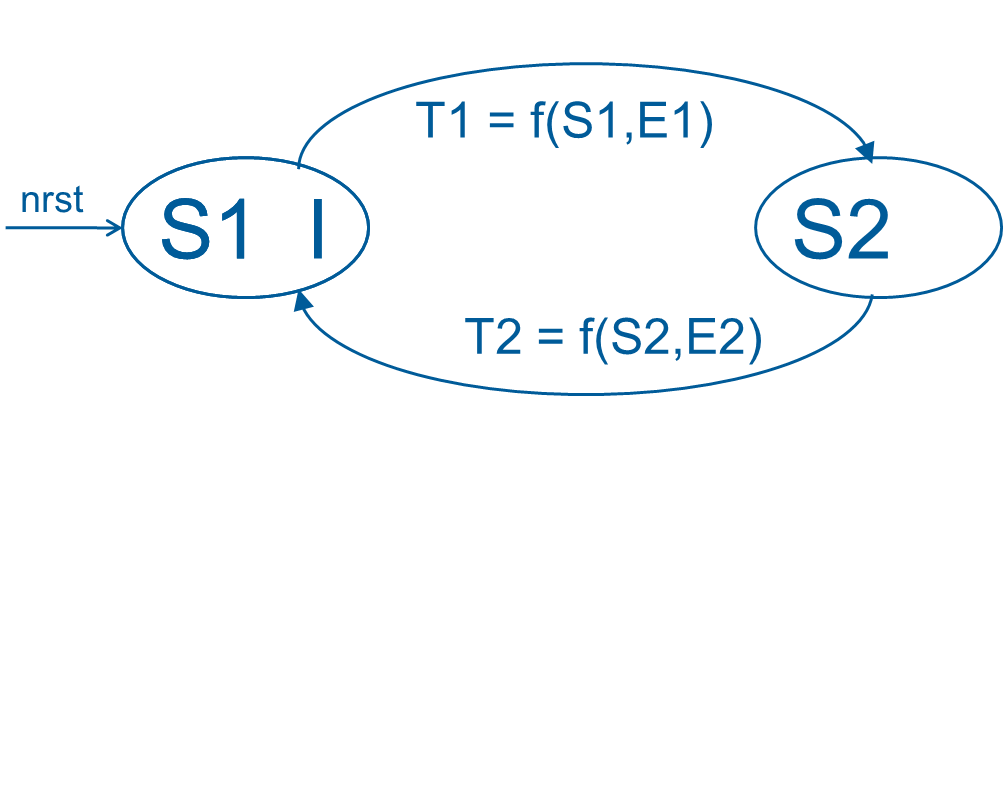
\includegraphics[width=0.25\textwidth]{pics/seq_uml}\\
			\begin{itemize}
			  \setlength{\itemsep}{1pt}
			  \setlength{\parskip}{0pt}
			  \setlength{\parsep}{0pt}
			  
			  \item S: Menge der Zust"ande mit Zustandsaktionen
			  \item $I\subseteq S:$ Initalzust"ande
			  \item T: "Ubergangsrelation $f(S,E)$
			  \item E: Eing"ange
			\end{itemize}
			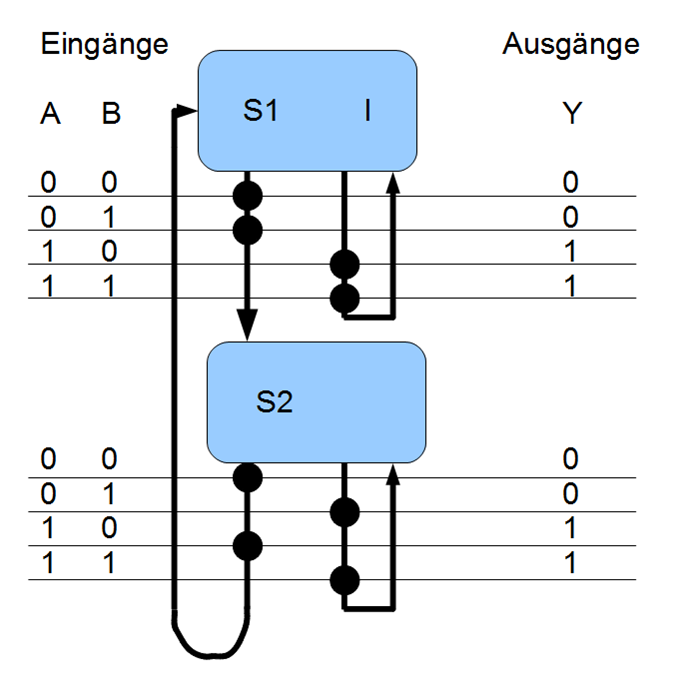
\includegraphics[width=0.25\textwidth]{pics/seq_statediagramm}\\
			\textbf{Vorgehen}
			\begin{enumerate}
			  \setlength{\itemsep}{1pt}
			  \setlength{\parskip}{0pt}
			  \setlength{\parsep}{0pt}
			
			  \item Zust"ande zeichnen und benennen
			  \item Initalzustand bestimmen
			  \item Eing"ange systematisch auflisten
			  \item Zustands"uberg"ange (Transitionen) bestimmen
			  \item Ausg"ange einzeichnen
			\end{enumerate}
	\end{multicols}
	\subsubsection{Zustandstabelle}\label{zustandstabelle}
	\begin{multicols}{3}
			\textbf{Vorgehen}
			\begin{enumerate}
			  \setlength{\itemsep}{1pt}
			  \setlength{\parskip}{0pt}
			  \setlength{\parsep}{0pt}
			
			  \item Ausgangspunkt = Warheitstabelle\\
			  \item Wird pro Zustand aufgeschrieben\\
			  \item Erg"anzt mit Folgezustand\\
			\end{enumerate}
		
			\begin{tabular}{|l|l|l|}
				\multicolumn{3}{c}{\textbf{Eingangsvariable}}\\
				\hline
				$In_1$ & $In_2$ & $\cdots$ \\
				\hline
				0 & 0 & $\cdots$ \\
				\hline
				0 & d & $\cdots$ \\
				\hline
				$\cdots$ & $\cdots$ & $\cdots$ \\
				\hline
			\end{tabular}
			
			\begin{tabular}{|l|l|l|}	
				\multicolumn{3}{c}{\textbf{Ausgangsvariable}}\\
				\hline
				$In_1$ & $In_2$ & $\cdots$ \\
				\hline
				0 & 0 & $\cdots$ \\
				\hline
				0 & d & $\cdots$ \\
				\hline
				$\cdots$ & $\cdots$ & $\cdots$ \\
				\hline
			\end{tabular}
	\end{multicols}			

\subsection{Zustandcodes}\label{zustandcodes}
	\begin{multicols}{2}
	\begin{itemize}
		\setlength{\itemsep}{1pt}
		\setlength{\parskip}{0pt}
		\setlength{\parsep}{0pt}
			
		\item Zust�nde werden der Reihe nach bin�r durch nummeriert.
		\item Ben�tigte Anzahl Speicherstellen $k$ f�r eine Anzahl Zust�nder $p$:\\
		$p\leq 2^k$ | $k=\log_2(p)=\frac{\log_{10}(p)}{\log_{10}(2)}$
		\item Anzahl M�glicher Speicherstellen:\\
		$q=\frac{(2^k)!}{(2^k-p)!}$
		\item \textbf{Alternative:} Graycode, es wechselt nur 1 Bit\\
	\end{itemize}
	\end{multicols}
	
\subsubsection{ONE-HOT Zustandscodierung}
	Pro Code wird genau eine Speicherstelle TURE. Alle anderen werden FALSE.
\subsubsection{ONE-COLD Zustandscodierung}
	Pro Code wird genau eine Speicherstelle FALSE. Alle anderen werden TRUE.
	
\subsection{Sequentielle Systeme in VHDL}
\lstinputlisting[language=VHDL,tabsize=2]{code/sequentiell.vhdl}

